\documentclass{article}
\usepackage{graphicx}
\usepackage{amsmath,amssymb}
\setlength{\parindent}{0pt}
\usepackage{listings}
\usepackage{lmodern}  % for bold teletype font
\usepackage{amsmath}  % for \hookrightarrow
\usepackage{xcolor}   % for \textcolor
\usepackage[a4paper,margin=1in,footskip=0.25in]{geometry}
\usepackage{graphicx}

\lstset{
  basicstyle=\ttfamily,
  columns=fullflexible,
  frame=single,
  breaklines=true,
}

\begin{document}

\title{Deep Reinforcement Learning Project 1 : Navigation}
\author{Rachel Schlossman}

\maketitle

\section{Learning Algorithm}
The learning algorithm is an implementation of a deep-Q network (DQN) as described in \cite{mnih2015human}. Following this paper, the action-values, $Q$, in iteration $i$ are updated using the following loss function:

\begin{equation}\label{eqn:loss}
L_i (\theta_i) = \mathbb{E}_{(s,a,r,s') \sim U(D)} \left[ \left( r + \gamma \max_{a'} Q(s',a';\theta_i^{-}) - Q(s,a;\theta_i) \right)^2 \right]
\end{equation}

where $\gamma$ is the discount factor . The minibatches of (state, action reward, next state) experiences, $(s, a, r, s') \sim U(D)$ are sampled uniformly from a replay buffer. The variable $\theta^{-}_i$ are the target network parameters. The target network parameters are set to the local Q-network parameters, $\theta_i$, every $N$ timesteps. Eqn. \ref{eqn:loss} is implemented in the \textit{learn} function using Python and Pytorch as follows: 

\begin{lstlisting}[language=Python]
    def learn(self, experiences, gamma):
        """Update value parameters using given batch of experience tuples.

        Params
        ======
            experiences (Tuple[torch.Variable]): tuple of (s, a, r, s', done) tuples 
            gamma (float): discount factor
        """
        states, actions, rewards, next_states, dones = experiences

        ## TODO: compute and minimize the loss
        Q_target_next_states = self.qnetwork_target(next_states).detach().max(1)[0].unsqueeze(1)
        
        # target component of loss
        # Q_des = r + gamma * max_{a'} Q(s',a',w-)
        
        Q_des = rewards + (gamma * Q_target_next_states) * (1-dones)
        
        # Q_actual
        # Q(s,a,w)
        Q_act = self.qnetwork_local(states).gather(1,actions)

        # Compute loss
        # L = (r + gamma * max_{a'} Q(s',a',w-) - Q(s,a,w))^2
        loss = F.mse_loss(Q_des, Q_act)
        # Minimize loss
        self.optimizer.zero_grad()
        loss.backward()
        self.optimizer.step()
        
        # update target network
        self.soft_update(self.qnetwork_local, self.qnetwork_target, TAU)
\end{lstlisting}

\subsection{Hyperparameters}
The following heperparameters were used in the DQN implementation:

\begin{itemize}
\item  $\gamma$ = 0.995
\item $N$ = 4
\item learning rate = 5e-4
\item replay buffer size  = 1e5
\item minibatch size = 64
\item time constant for soft update of target parameters, $\tau$ = 1e-3
\end{itemize}


\section{Model Architecture}
The input passes through two linear layers with relu activation followed by a linear output layer. The two hidden layers each are comprised of 64 nodes. The code implementation is shown below. 

\begin{lstlisting}[language=Python]
class QNetwork(nn.Module):
    """Actor (Policy) Model."""

    def __init__(self, state_size, action_size, seed,
                h1_units=64, h2_units=64):
        """Initialize parameters and build model.
        Params
        ======
            state_size (int): Dimension of each state
            action_size (int): Dimension of each action
            seed (int): Random seed
            h1_units (int) : width of 1st hidden layer
            h2_units (int) : width of 2nd hidden layer
        """
        super(QNetwork, self).__init__()
        self.seed = torch.manual_seed(seed)
        # fc stands for "fully connected"
        self.fc1 = nn.Linear(state_size, h1_units)
        self.fc2 = nn.Linear(h1_units, h2_units)
        self.fc3 = nn.Linear(h2_units, action_size)

    def forward(self, state):
        """Build a network that maps state -> action values."""
        o1 = F.relu(self.fc1(state))
        o2 = F.relu(self.fc2(o1))
        o3 = self.fc3(o2)
        
        return o3
\end{lstlisting}

\section{Results}
The agent is able to receive an average reward over 100 episodes of +13 in 395 episodes, as shown in Fig. \ref{fig:results}.

\begin{figure}[ht]
\centering
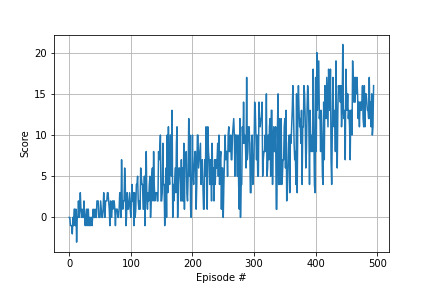
\includegraphics[scale=0.75]{./figures/results.png}
\caption{Average Score Plot}
\label{fig:results}
\end{figure}

\section{Future Work}
The learning algorithm does not make use of Double Q-Learning, prioritized experience replay, or a dueling DQN architecture. Using one or more of these modifications could potentially improve the performance of the DQN agent. 

\bibliographystyle{plain}
\bibliography{bib}

\end{document}